\chapter{Schedule and Timeline}

The original CHSR timeline, drafted in 2008, proposed an “electrified commuter service as soon as 2020” \citep{ureport2015}. However, cost overruns, environmental lawsuits, and delays in right-of-way land acquisition forced the CHSR authority to push its expected start date to 2030. This had led to public scrutiny and a decline in the public’s interest in the project. Phase 1 now targets the completion of the Merced to Bakersfield segment by 2030 \citep{ureport2023}, with further safety enhancements scheduled for 2040 \citep{ureport2025}.

\section{Schedule Management Challenges}
Various challenges have impacted the CHSR schedule:
\begin{itemize}
	\item Legal delays due to land disputes and environmental litigation \citep{pur2025}.
	\item Inflation and supply chain disruptions post-COVID-19.
	\item Slow utility relocation and coordination with local jurisdictions.
	\item Delays in federal approvals and funding disbursements.
\end{itemize}

\section{Gantt Chart \citep{ureport2025}}
\noindent \centering
\vspace*{1em}
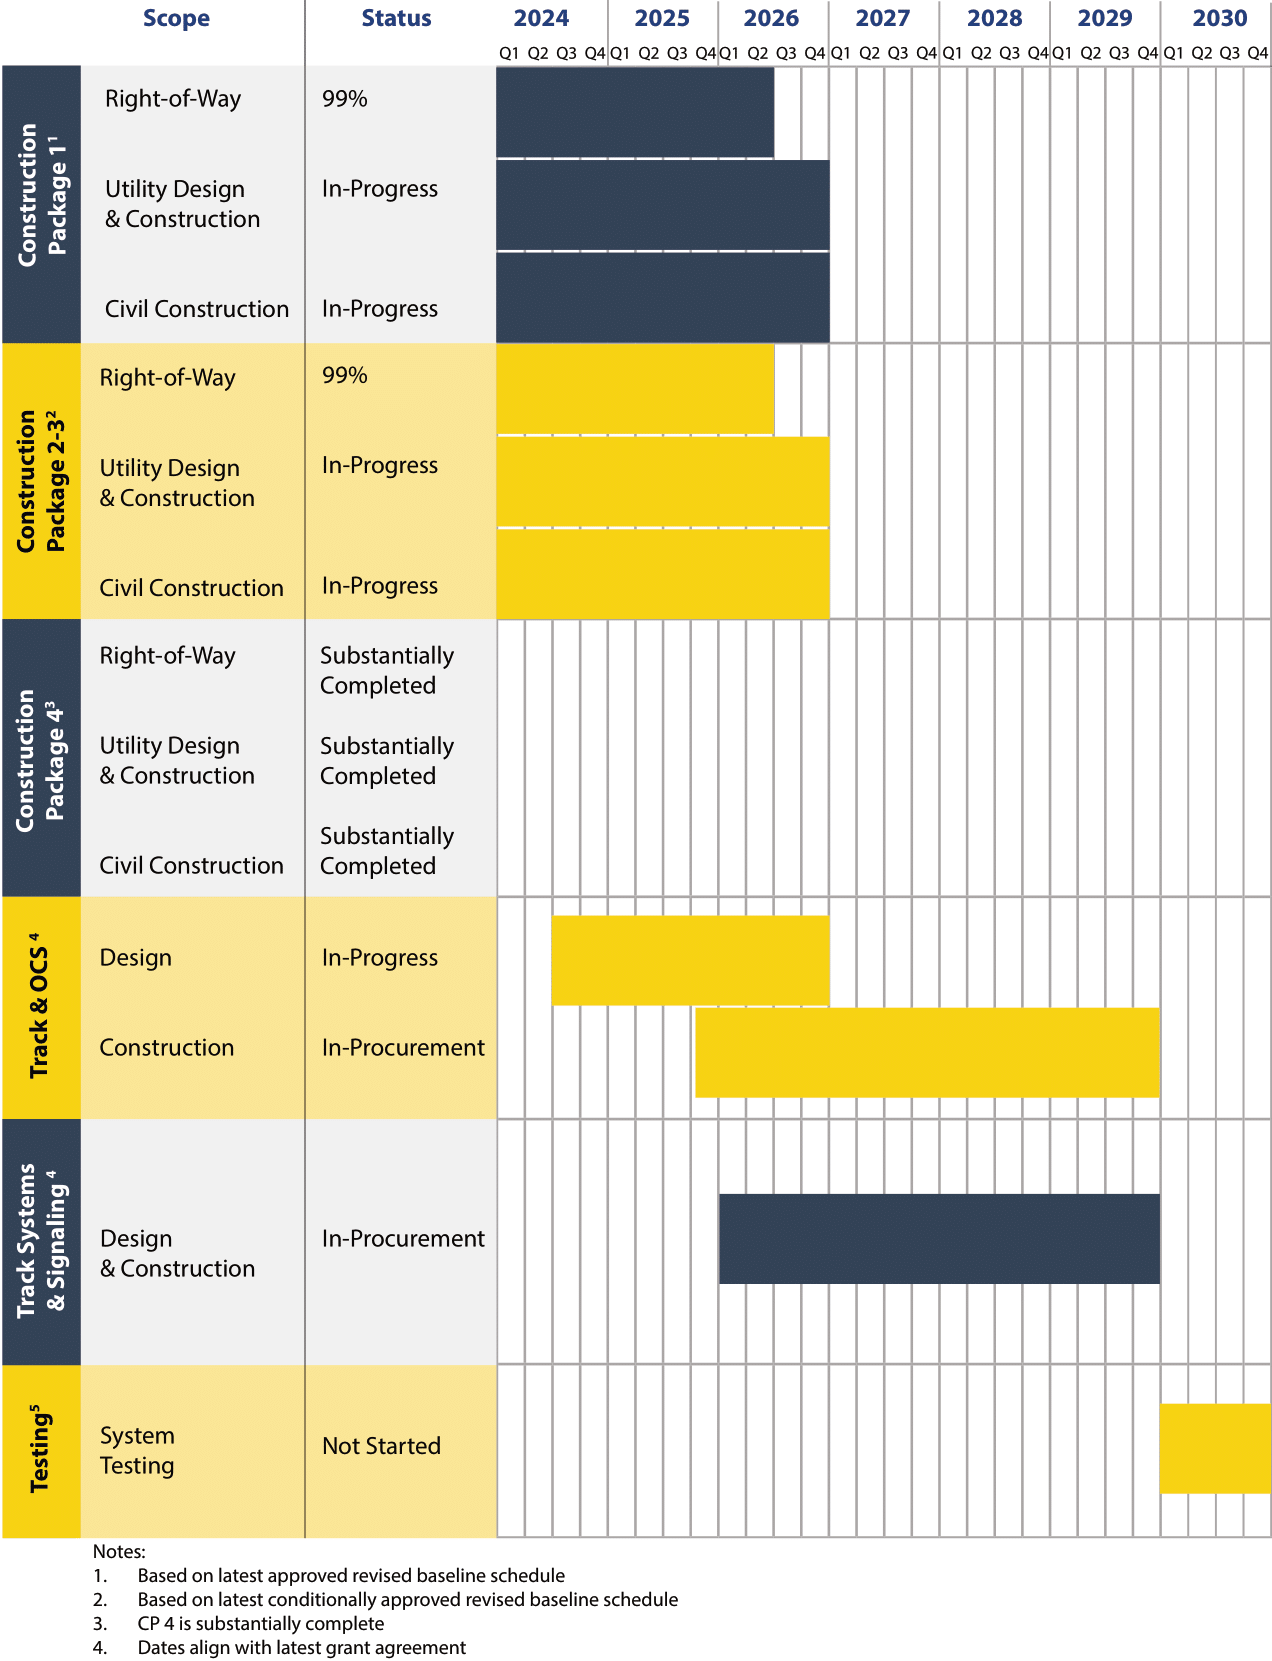
\includegraphics[width=\linewidth]{./attachments/timeline}
\justifying

\section{Major Milestones}
\parindent20pt In 2024, “[Construction Package (CP)] 4 reached substantial completion, highlighting tremendous progress toward civil construction in the Central Valley” \citep{ureport2025}. Construction packages one, two, and three are expected to be finished in 2026, with the Track Systems, Signaling, and Overhead Contact System (OCS) following closely behind, with completion dates set as late as 2029. Testing is scheduled to begin in 2030, with the project’s launch expected to follow in the same year. These milestones demonstrate a phased delivery model designed to maximize project resilience and flexibility in the face of changing political and economic conditions. \par